\chapter{Prolego: A máquina de raciocínio}

Este capítulo traz o detalhamento dos componentes que integram o Prolego, bem como a descrição da montagem do robô, do tapete, das missões, da arquitetura do robô e do Prolego. Este capítulo aborda ainda a configuração do ambiente e a integração do Prolego com o Traveller.

\section{Contextualização}

A proposta deste trabalho foi a construcão de uma máquina de raciocínio, utilizando programação dinâmica e implementada na linguagem Prolog, que fosse capaz de gerar um roteiro de missões otimizado, isto é, que conseguisse a maior pontuação em um determinado tempo. As entradas da máquina de raciocínio são: o tempo total para a execução das missões e uma base de conhecimento que contém as missões ainda não realizadas.
A partir dessas entradas, a máquina de raciocínio avalia quais missões devem ser executadas para que se alcance a quantidade máxima de pontos possível. A base de conhecimento contendo as missões a serem executadas foi implementada seguindo a seguinte estrutura:
 \begin{lstlisting} 
 missao(Valor, Tempo).
 \end{lstlisting}
 Desta forma, o Prolego avalia o valor e o tempo, em segundos, para executar cada missão. Visando limitar o escopo de atuação, foram estabelecidos alguns pontos para este trabalho:
 \begin{itemize}
 \item toda missão tem início no ponto X = 0 e Y = 0 e, a ele, deve retornar, pois se tal limitação não fosse estabelecida, o tempo para execução de cada missão seria variável de acordo com a localização;
 \item para contabilizar a pontuação da missão, não foram consideradas possíveis penalidades;
 \item o tempo total da missão é igual ao tempo de deslocamento (tempo necessário pro robô sair do ponto inicial e chegar ao ponto final) somado ao tempo de execução da missão;
 \item o tempo de deslocamento da missão foi medido utilizando o caminho gerado pelo Traveller de acordo com os pontos inicial e final de cada missão, e
 \item o tempo de execução da missão foi uma estimativa, considerando o tempo que o robô leva para fazer o movimento acrescido de uma margem de erro de 2 segundos. Para estimar esse tempo, foram analisados alguns vídeos\footnote{https://www.youtube.com/channel/UCDWIi63k2Io4hFEag19QE0Q}\footnote{https://www.youtube.com/channel/UCd1jb1c\-i3ERC\_5V1Qo3LGw} de competição da turma de Princípios de Robótica Educacional da UnB - Faculdade Gama. 
 \end{itemize}
 A Figura \ref{ComunicacaoProlegoTraveller} demonstra a comunicação entre: o Prolego, o Traveller e os módulos do Traveller entre si.

 \FloatBarrier
\begin{figure}[!h]
\centering
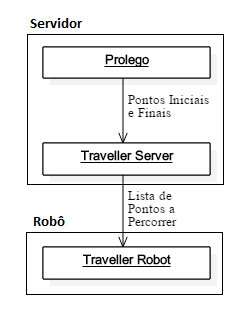
\includegraphics[keepaspectratio=true,scale=0.7]{figuras/Comunicacao_Prolego_Traveller.png}
\caption{Comunicação entre o Prolego e o Traveller Framework}
\label{ComunicacaoProlegoTraveller}
\end{figure}
 
 
 Inicialmente, o Prolego seria hospedado no robô mas, como se pode observar na Figura \ref{ComunicacaoProlegoTraveller}, a comunicação do mesmo é feita com o módulo Server do Traveller. Logo, por questão de otimização, o Prolego ficou hospedado no servidor e a comunicação com o robô é realizada via \textit{Bluetooth}.

\section{Arquitetura do robô}\label{arquiteturaDoRobo}
\apud{vieira2005controle}{rinconframework} define uma arquitetura para robôs móveis baseada em cinco camadas: percepção, decisão, planejamento de caminho, geração de trajetória e sistema de controle. Essa arquitetura pode ser visualizada na Figura \ref{arquiteturaCamadas}.

\FloatBarrier
\begin{figure}[!h]
\centering
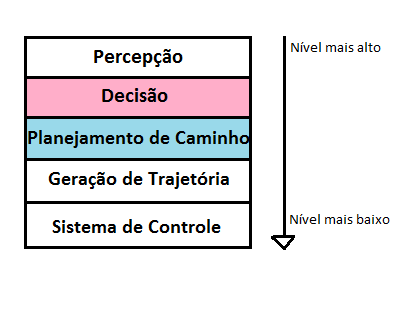
\includegraphics[keepaspectratio=true,scale=0.7]{figuras/arquiteturaCamadas.png}
\caption{Arquitetura em camadas de robôs móveis - \apud{vieira2005controle}{rinconframework}}
\label{arquiteturaCamadas}
\end{figure}

A primeira camada, denominada Camada de Percepção, trata da percepção do robô acerca do mundo ao seu redor, utilizando os sensores que o compõe. Essa camada é responsável, por exemplo, por identificar os obstáculos contidos no tapete. Neste trabalho, os obstáculos foram mapeados manualmente.

A segunda camada, denominada Camada de Decisão, é a responsável por decidir as ações que o robô irá executar. Esta camada é o cerébro do robô, sendo nela que o trabalho proposto age. A máquina de raciocínio que atua nesta camada tem o cálculo da trajetória, definida na 	quarta camada, através do \textit{framework} Traveller. Com o tempo da trajetória conhecida e somado ao tempo de execução da missão, tem-se o tempo total da missão, e a máquina de raciocínio decide quais missões devem ser executadas.

A terceira camada define a trajetória que o robô irá executar para chegar à posição desejada, é nessa camada que o \textit{framework} Traveller age. Com o conhecimento do ambiente, anteriormente levantado pela Camada de Percepção, o Traveller define um percurso por onde o robô deve seguir para não colidir com nenhum obstáculo.

A quarta camada recebe o plano da trajetória feito pela camada anterior e define quais ações devem ser feitas sobre o \textit{hardware} para executar o plano. Essa camada tem conhecimento das dimensões e limitações do robô. A última camada atua diretamente no \textit{hardware} para garantir que os atuadores estão recebendo o sinal e agindo conforme planejado.
 
\section{Montagem do robô}
O robô utilizado por este trabalho é o Bauen, um tipo de montagem do robô NXT. Nessa montagem, o robô é feito com três motores, dois para as esteiras e um preparado para receber uma garra ou outro adereço. O motor da esquerda deve ser ligado na porta B, o da direita na porta C e o da "garra" na porta A. O tutorial completo, contendo o passo-a-passo para a montagem do robô pode ser encontrado no site da LEGO\footnote{$http://lego.brickinstructions.com/lego_instructions/set/8547/Mindstorms_NXT_2.0$}. 

Na Figura \ref{bauen}, é possível visualizar a aparência do robô quando montado. 

\FloatBarrier
\begin{figure}[!h]
\centering
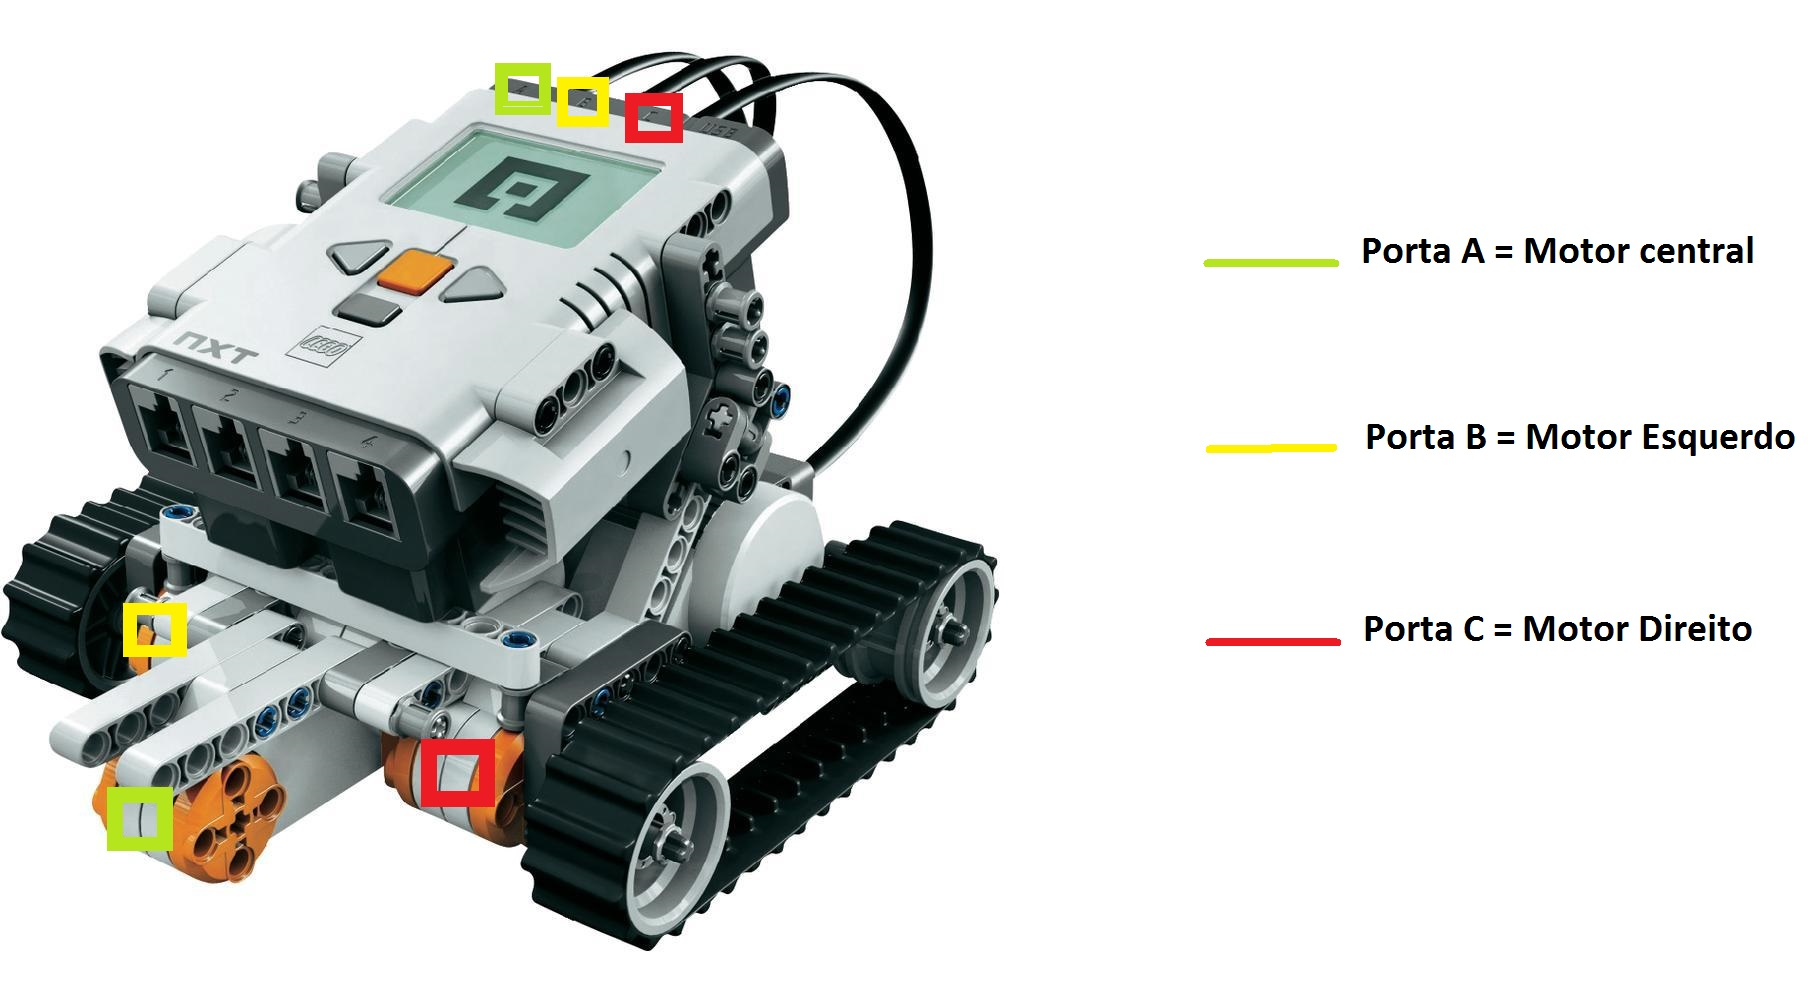
\includegraphics[keepaspectratio=true,scale=0.15]{figuras/bauen.jpg}
\caption{Montagem do robô Bauen - Lego Mindstorms NXT}
\label{bauen}
\end{figure}


\section{Tapete de missões} \label{tapeteDeMissoes}
O tapete de missões escolhido para esse trabalho é o \textit{Nature's Fury} \cite{challengeFury}, utilizado como desafio do torneio \textit{First Lego League} de 2013, que tem como temática uma tsunami que está devastando as cidades. Esse tapete tem caráter educacional, ensinando quanto aos lugares seguros e não seguros para permanecer quando uma tsunami está em atividade. Os lugares seguros durante uma tsunami, demarcados no tapete, são bonificados com uma pontuação extra, caso o robô fique nesse lugar. Já os lugares inseguros também são demarcados no tapete. Porém, esses lugares representam penalidades, com perda de pontuação, caso o robô passe pelos mesmos. Existem missões de salvar os animais de estimação, salvar pessoas, levar água e mantimentos para os lugares seguros.
O tapete \textit{Nature's Fury} foi escolhido para ser objeto de estudo deste projeto, uma vez que é utilizado nas aulas de Princípios de Robótica Educacional, sendo assim, mais acessível do que outros tapetes. Na Figura \ref{natureFury}, é possível visualizar o tapete, bem como os obstáculos que possui. 

\FloatBarrier
\begin{figure}[!h]
\centering
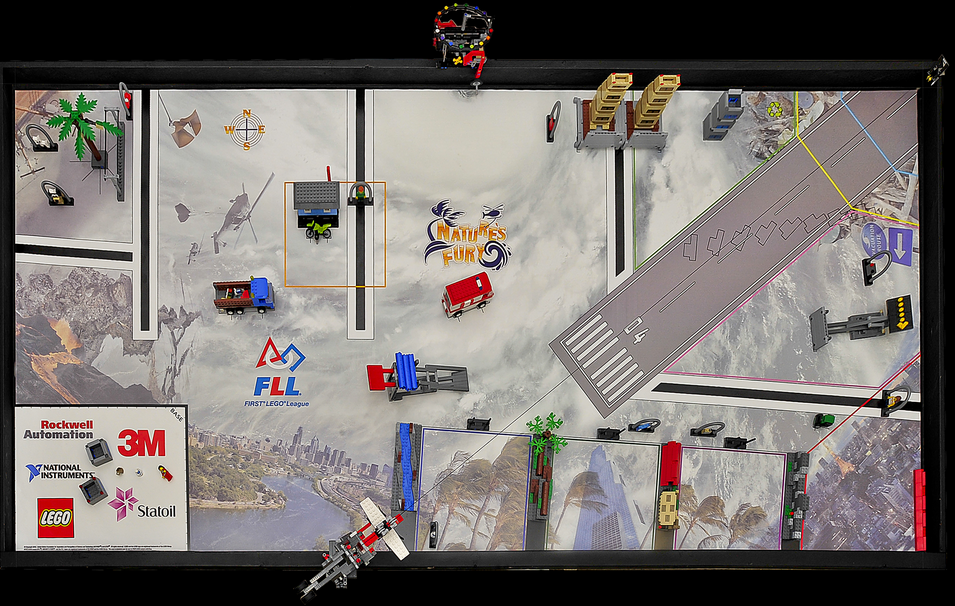
\includegraphics[keepaspectratio=true,scale=0.5]{figuras/natureFury.png}
\caption{Tapete de missões \textit{Nature's Fury} - Lego Mindstorms NXT}
\label{natureFury}
\end{figure}

 
\section{Descrição das missões}
As missões contidas no tapete \textit{Nature's Fury} \cite{challengeFury} são descritas a seguir:
\begin{itemize}
\item \textbf{missão caminhão de fornecimento:} consiste em levar o caminhão até a área amarela do mapa. Pontuação: 20 pontos;
\item \textbf{missão sinal de evacuação:} consiste em levantar a placa com o sinal de evacuação. Pontuação: 30 pontos;
\item \textbf{missão avião de carga:} consiste em fazer o avião chegar à área azul ou amarela do tapete. Pontuação: 20 pontos para a área amarela, 30 pontos para a área azul;
\item \textbf{missão galho da árvore:} consiste em retirar o galho da árvore sem deixá-lo encostar nos fios de alta tensão. Pontuação: 30 pontos;
\item \textbf{missão tsunami:} consiste em fazer com que as três ondas que estão suspensas toquem o tapete. Pontuação: 20 pontos;
\item \textbf{missão ambulância:} consiste em levar a ambulância até a área amarela do tapete. Pontuação: 25 pontos;
\item \textbf{missão pista limpa:} consiste em retirar qualquer objeto da pista de pouso. Pontuação: 30 pontos;
\item \textbf{missão realocação de construção:} consiste em retirar todas as peças cinzas encontradas na construção da área verde do tapete. Pontuação: 20 pontos;
\item \textbf{missão teste da base de isolamento:} consiste em encostar na base de isolamento e derrubar apenas um dos prédios. Pontuação: 30 pontos;
\item \textbf{missão construção:} consiste em empilhar os segmentos na área rosa do tapete. Pontuação: 5 pontos para cada segmento empilhado;
\item \textbf{missão obstáculo:} consiste no robô passar por cima de obstáculos chegando às áreas coloridas do tapete. Nesse caso, para cada cor do tapete, existe uma pontuação. Pontuação: 10 pontos para a área azul, 16 pontos para a área verde, 23 pontos para a área roxa e 31 pontos para a área vermelha;	
\item \textbf{missão elevar a casa:} consiste no robô abaixar a alavanca que eleva a casa. Pontuação: 25 pontos;
\item \textbf{missão progresso:} consiste em rodar um círculo de cores. Pontuação: 2 pontos para cada cor que o ponteiro passar;
\item \textbf{missão família:} consiste em juntar as pessoas que estão no tapete em uma única área colorida. Pontuação: 33 para duas pessoas juntas, ou 66 para 3 pessoas juntas;
\item \textbf{missão água:} consiste em juntar ao menos uma pessoa com uma garrafa de água na mesma região. Pontuação: 15 pontos para cada pessoa+água;
\item \textbf{missão segurança:} consiste em levar pelo menos uma pessoa à região vermelha ou amarela do tapete. Pontuação: 12 pontos para cada pessoa na área amarela ou 18 pontos para cada pessoa na área vermelha;
\item \textbf{missão \textit{pets}:} consiste em juntar ao menos um animal à uma pessoa numa área colorida. Pontuação: 15 pontos para cada pet+pessoa;
\item \textbf{missão equipamentos e suprimentos:} consiste em levar pelo menos um item, exceto a água, para a região vermelha ou amarela do tapete. Pontuação: 3 pontos para cada item na área amarela ou 4 pontos para cada item na área vermelha, e
\item \textbf{missão lugar seguro:} consiste no robô estar na região vermelha no final do jogo. Pontuação: 25 pontos. 
\end{itemize}

\section{Configuração do Ambiente}
	O Sistema Operacional escolhido para ser utilizado por esse trabalho foi o Windows, mais especificamente a versão 10. Foi utilizada a IDE Eclipse para trabalhar com a parte Java do projeto, e o editor NotePad++ para trabalhar com a parte Prolog do Projeto. O compilador Prolog utilizado foi o SwiProlog, e o executável pode ser baixado no próprio site\footnote{http://www.swi-prolog.org/download/stable}. 
	
	Para trabalhar com o Java, foi necessário instalar o Java 7, obrigatoriamente na versão de 32 bits, pois o Lego não aceita a versão 64bits. Da mesma forma, o Eclipse teve que ser instalado na versão 32 bits.
	O NXT tem um \textit{firmware} específico para se trabalhar com o Java, chamado leJOS. A instalação do leJOS deve ser feita no computador, no eclipse e no robô. Tais configurações são descritas a seguir.

	\textbf{Instalação do leJOS no Windows}

	O executável pode ser baixado no próprio site do leJOS\footnote{http://www.lejos.org/}, na versão 0.9.1 . Ao final da instalação do executável, é iniciado o NXJ Flash, aplicativo responsável por instalar o \textit{firmware} do leJOS no robô, como mostra a Figura \ref{lejosFinish}.
\FloatBarrier
\begin{figure}[!h]
\centering
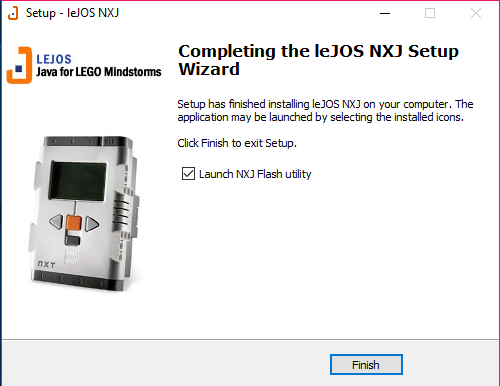
\includegraphics[keepaspectratio=true,scale=0.7]{figuras/lejosFinish.png}
\caption{Instalação do leJOS no Windows}
\label{lejosFinish}
\end{figure}

	\textbf{Instalação do leJOS no Robô}

	O aplicativo NXJ Flash, instalado pelo executável do leJOS, é o responsável pela instalação do \textit{firmware} no robô. Para iniciar a instalação, é necessário que o robô esteja conectado ao computador via cabo USB, ou seja, a instalação não é feita via \textit{bluetooth}.  
	A Figura \ref{lejosFirmware} mostra a aplicação NXJ Flash.
\FloatBarrier
\begin{figure}[!h]
\centering
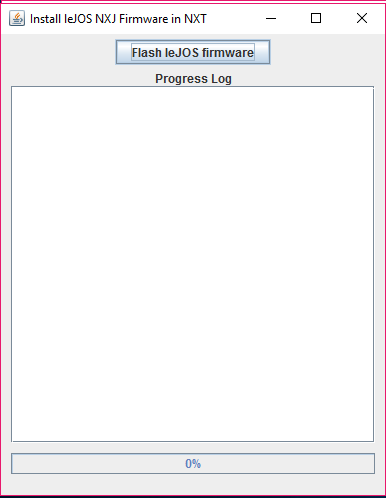
\includegraphics[keepaspectratio=true,scale=0.7]{figuras/lejosFirmware.png}
\caption{Aplicativo NXJ Flash}
\label{lejosFirmware}
\end{figure}
	Ao clicar no botão \textit{Flash leJOS Firmware}, mostrado na Figura \ref{lejosFirmware}, é iniciada a instalação do \textit{firmware} no robô.
	
	\textbf{Instalação do leJOS no Eclipse}
	
	O leJOS para o Eclipse é um \textit{plugin}, que é instalado clicando na aba \textit{Help}, no Eclipse, na opção \textit{Install New Software}. A Figura\ref{installNewSoftware} mostra a janela para instalação do \textit{plugin}. 

\FloatBarrier
\begin{figure}[!h]
\centering
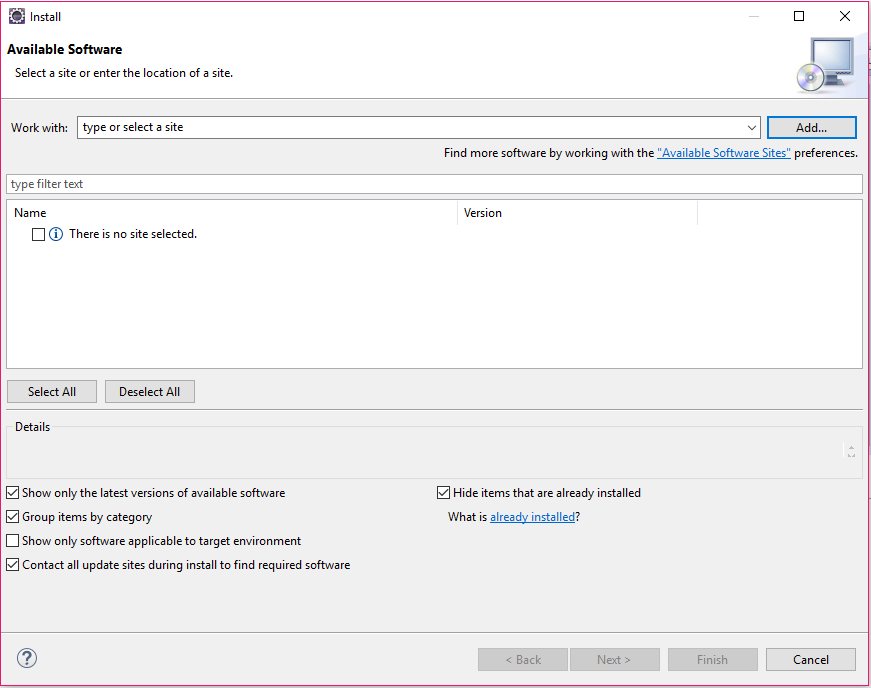
\includegraphics[keepaspectratio=true,scale=0.7]{figuras/installNewSoftware.png}
\caption{Instalando Plugin no Eclipse}
\label{installNewSoftware}
\end{figure}
	
	Ao clicar em \textit{add}, um pop-up é aberto com as opções \textit{name} e \textit{url}, que devem ser preenchidas como mostrado na Figura \ref{pluginNXJ}. Nesse caso, basta clicar em OK, selecionar o \textit{plugin}, e clicar em \textit{Finish}.  

\FloatBarrier
\begin{figure}[!h]
\centering
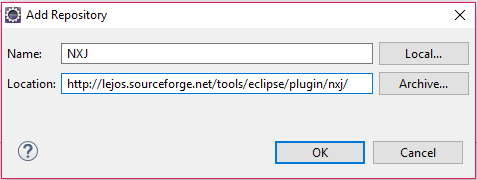
\includegraphics[keepaspectratio=true,scale=0.7]{figuras/pluginNXJ.png}
\caption{Dados do Plugin do leJOS}
\label{pluginNXJ}
\end{figure}
	
	Para finalizar, é necessário adicionar o caminho, a partir do qual o leJOS foi instalado, na variável NXJ\_HOME, encontrada na aba \textit{Window}, opção \textit{Preferences}, clicando em leJOS NXJ, conforme mostrado na Figura \ref{nxjhome}.
		
\FloatBarrier
\begin{figure}[!h]
\centering
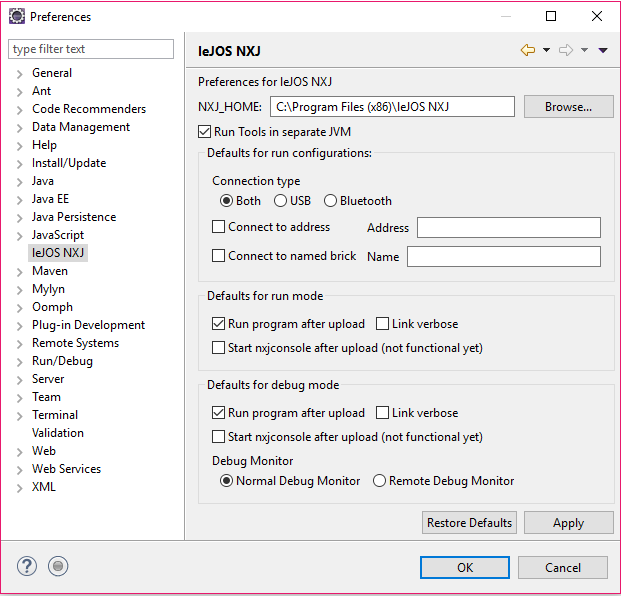
\includegraphics[keepaspectratio=true,scale=0.7]{figuras/NXJHOME.png}
\caption{Caminho do NXJ HOME}
\label{nxjhome}
\end{figure}
	
	
	
\section{Arquitetura do Prolego}\label{arquiteturaProlego}
	A arquitetura do robô costuma ser em camadas, e o Prolego age na camada de decisão, como mostrado na Seção \ref{arquiteturaDoRobo}. Porém, a arquitetura interna do Prolego é componentizada, onde a \textit{Main} controla todos os outros de forma hierárquica, como mostra o diagrama da Figura \ref{DiagramaArvoreInicial}. Para melhor visualização, esse diagrama foi elaborado em ramos, sendo esses descritos nas Figuras \ref{DiagramaRamo1}, \ref{DiagramaRamo2}, \ref{DiagramaRamo3}, \ref{DiagramaRamo4}.
	
\FloatBarrier
\begin{figure}[!h]
\centering
\includegraphics[keepaspectratio=true,scale=0.7]{figuras/DiagramaArvoreInicial.png}
\caption{Diagrama de Fluxo do Prolego}
\label{DiagramaArvoreInicial}
\end{figure}


\FloatBarrier
\begin{figure}[!h]
\centering
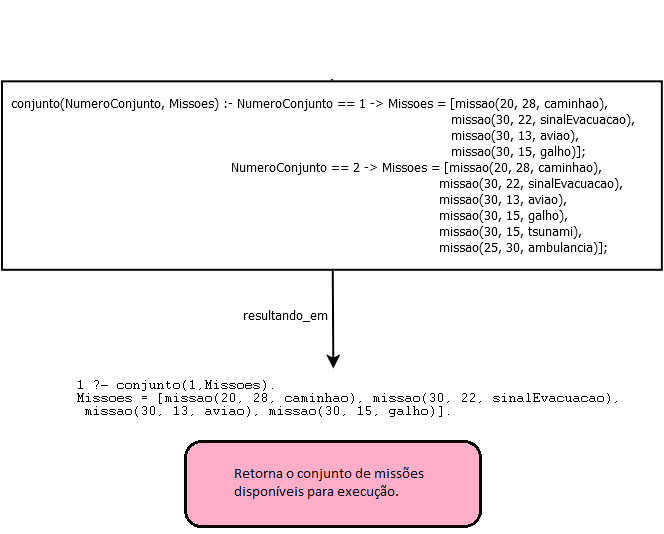
\includegraphics[keepaspectratio=true,scale=0.7]{figuras/DiagramaRamo1.png}
\caption{Diagrama de Fluxo do Prolego - Ramo 1}
\label{DiagramaRamo1}
\end{figure}


\FloatBarrier
\begin{figure}[!h]
\centering
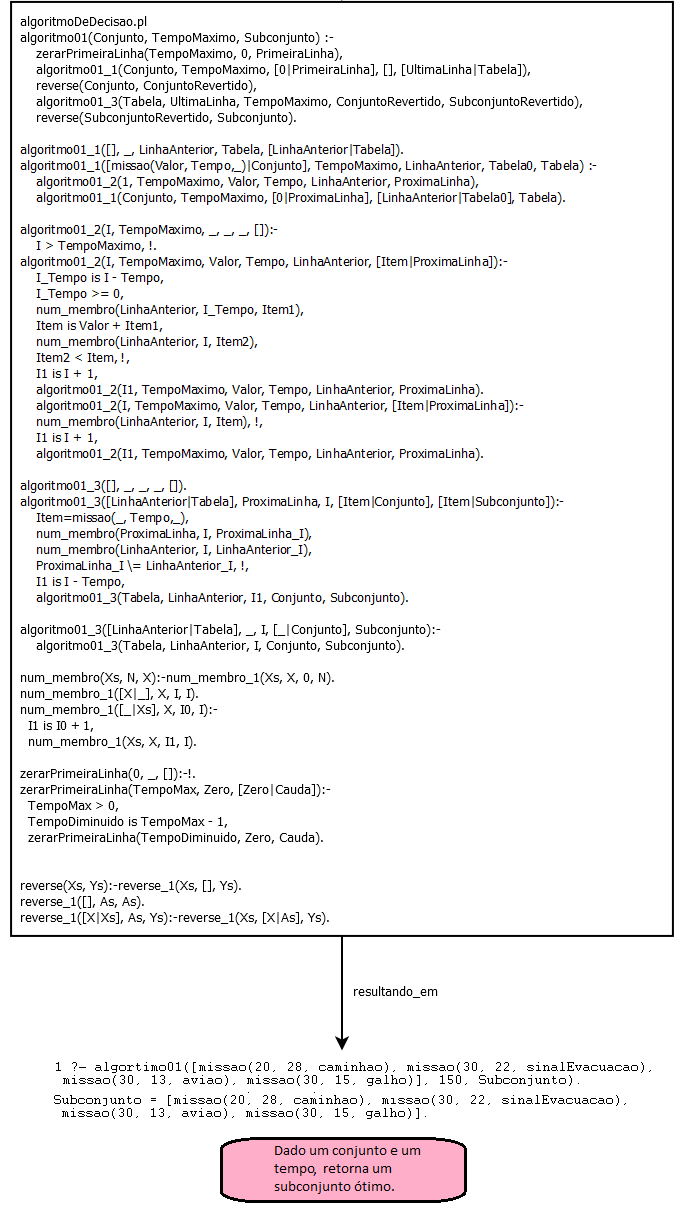
\includegraphics[keepaspectratio=true,scale=0.7]{figuras/DiagramaRamo2.png}
\caption{Diagrama de Fluxo do Prolego - Ramo 2}
\label{DiagramaRamo2}
\end{figure}



\FloatBarrier
\begin{figure}[!h]
\centering
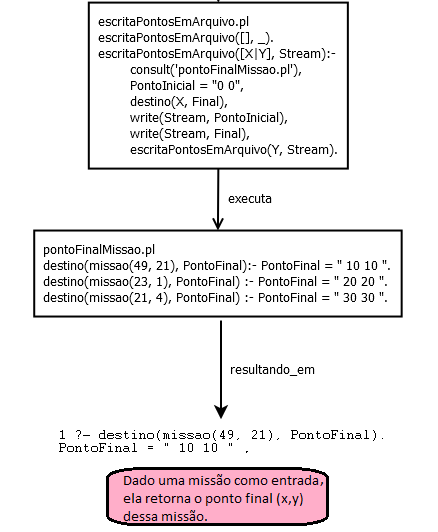
\includegraphics[keepaspectratio=true,scale=0.7]{figuras/DiagramaRamo3.png}
\caption{Diagrama de Fluxo do Prolego - Ramo 3}
\label{DiagramaRamo3}
\end{figure}



\FloatBarrier
\begin{figure}[!h]
\centering
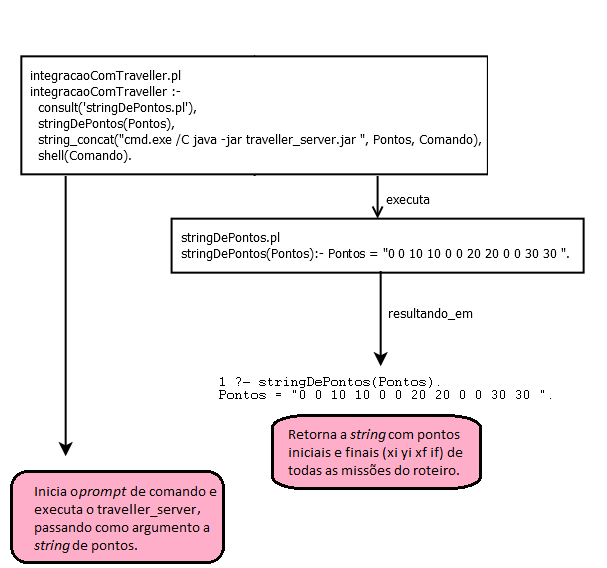
\includegraphics[keepaspectratio=true,scale=0.7]{figuras/DiagramaRamo4.png}
\caption{Diagrama de Fluxo do Prolego - Ramo 4}
\label{DiagramaRamo4}
\end{figure}


 
 As subseções a seguir explicam o comportamento de cada componente que compõe o Prolego.


\subsection{\textit{main}}
	O componente \textit{main} tem apenas uma regra chamada prolego. Esta regra é responsável por pegar o conjunto de missões da classe conjuntoDeMissoes.pl, de acordo com o número do conjunto passado; acionar o componente \textit{algoritmoDeDecisão.pl} passando, o conjunto juntamente com o tempo restante, e receber como retorno um subconjunto ótimo.
	
	Em posse desse subconjunto, a \textit{main} cria um arquivo para escrita, chamado \textit{stringDePontos.pl}, no qual a regra \textit{escritaDePontos} escreve os pontos iniciais e finais de todas as missões.
	A main, por fim, chama a regra \textit{integracaoComTraveller}, que é responsável por integrar o Prolego com o \textit{framework} Traveller.

\subsection{\textit{conjuntoMissoes}}
	Este componente contém as missões disponíveis para execução. Os conjuntos de missões estão associados a um número. Dependendo do número passado pelo usuário, para a regra \textit{prolego} do componente \textit{main}, tal componente retorna um conjunto diferente de missões. O componente \textit{conjuntoMissoes} pode conter 'n' conjuntos, a serem cadastrados pelo usuário.
	
\subsection{\textit{algoritmoDeDecisao}}
	Este componente é uma adaptação do conhecido problema da mochila. O componente recebe um conjunto de missões, e através de programação dinâmica avalia a pontuação e o tempo de cada missão, retornando então um subconjunto ótimo de missões a serem executadas.

\subsection{\textit{pontoFinalMissao}}
	Este componente contém o ponto final de todas as missões. Quando passado a missão, ee retorna o ponto final da mesma. Não é possível obter todos os pontos finais do conjunto de uma só vez, pois é possível consultar apenas uma missão por vez.
	
\subsection{\textit{escritaPontosEmArquivo}}
	Este componente recebe o subconjunto do componente \textit{main}, e de forma recursiva ele consulta o componente \textit{pontoFinalMissão} para obter o ponto final da missão avaliada. Para cada missão este componente escreve no arquivo os pontos iniciais e finais da mesma.

\subsection{\textit{stringDePontos}}
	Este é um componente criado em tempo de execução, com os pontos iniciais e finais do subconjunto ótimo. Ele retorna uma \textit{string} com todos os pontos.
	
\subsection{\textit{integracaoComTraveller}}
	Este componente é responsável por inicializar o módulo Server do Traveller, passando a \textit{string} de pontos como argumento. Para inicializar o Traveller, este componente utiliza o método \textit{shell} que possibilita executar qualquer linha de comando. Desta forma, para rodar o Traveller, primeiramente, inicializou-se o \textit{prompt} de comando, e depois executou o \textit{.jar} da aplicação.

\section{Integração com o Traveller}
	A integração do Prolego com o Traveller foi efetuada em duas partes: a primeira foi a configuração do Traveller para trabalhar com o mapa e o robô definidos por este trabalho e a segunda foi a criação de métodos no Prolego para adaptar a saída à entrada do Traveller. Essas partes são descritar a seguir.
	
	A Figura \ref{criacaoMapa} mostra o mapa que foi colocado no Traveller, em forma de uma matriz booleana, onde  "1" representa que existe um obstáculo naquela célula, e "0" representa uma célula livre. Cada célula da matriz equivale a 3 centímetros do mapa real. Todo o mapeamento das células foi feito de forma manual.

\FloatBarrier
\begin{figure}[!h]
\centering
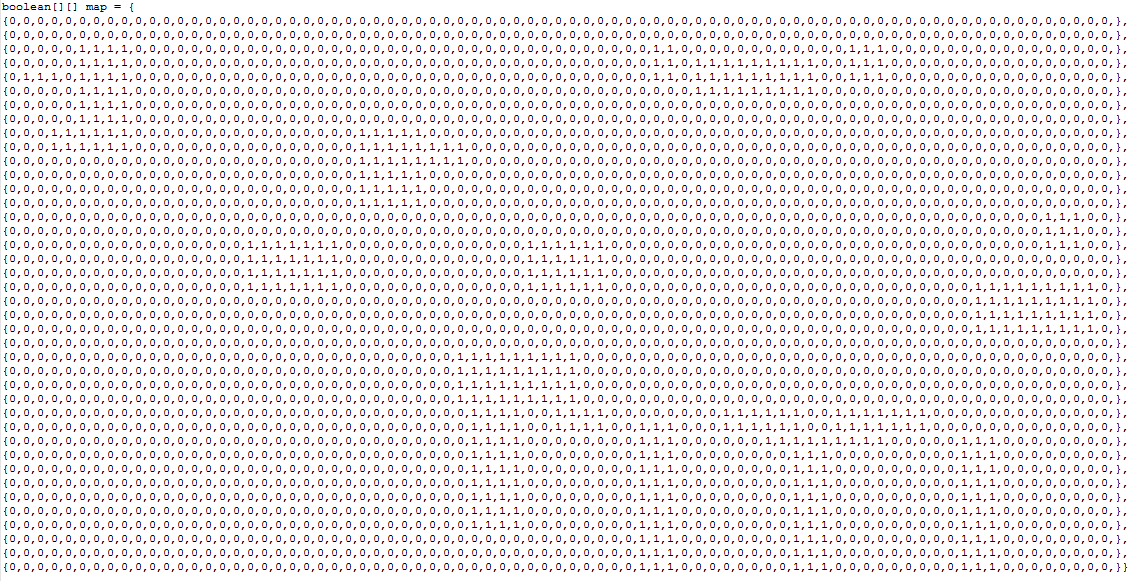
\includegraphics[keepaspectratio=true,scale=0.7, angle = 90]{figuras/criacaoMapa.png}
\caption{Método \textit{createMap} do classe \textit{Main} - Traveller Server}
\label{criacaoMapa}
\end{figure}

	A Figura \ref{configTravellerRobo} mostra o método \textit{attendRequest} da classe \textit{Main}. É nesse método que é especificado o tamanho do robô utilizado, no caso desse trabalho 17cm (o tamanho do robô é o maior tamanho entre a largura e o comprimento), o tamanho da célula do mapa, nesse caso é 3cm.

\FloatBarrier
\begin{figure}[!h]
\centering
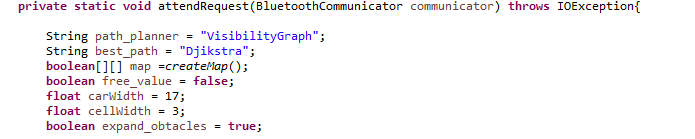
\includegraphics[keepaspectratio=true,scale=0.7]{figuras/configTravellerRobo.png}
\caption{Método \textit{attendRequest} da classe \textit{Main} - Traveller Server}
\label{configTravellerRobo}
\end{figure}

	Com essa configuração, o Traveller já tinha os dados necessários para criar o melhor caminho para o robô alcançar o ponto de destino, porém, ainda foi necessário configurar a conexão \textit{bluetooth} entre o Traveller e o NXT. 
	
	Para realizar a conexão, foi utilizado o próprio aplicativo de \textit{bluetooth} do computador, com o qual foi procurado e localizado o NXT. Ao emparelhar, foi utilizado o PIN 1234, que é o PIN do NXT. Este PIN pode ser modificado nas configurações do NXT por qualquer outro PIN de 4 dígitos.

	Realizado o emparelhamento, o Traveller já era capaz de enviar o código do Traveller Robot para o NXT, via \textit{bluetooth}.

	A segunda parte da integração foi a criação dos métodos \textit{escritaDePontosEmArquivos}, \textit{stringDePontos} e \textit{integracaoComTraveller}, no Prolego. Os dois primeiros métodos são responsáveis pela adaptação do retorno do \textit{algoritmoDeDecisao} para uma entrada válida para o Traveller, ou seja, uma \textit{string} com pontos iniciais e finais. O último método é responsável por inicializar o Traveller Server e passar os pontos para ele.
	
	Com essas duas etapas concluídas foram inicializados os cenários de teste.
	
\section{Considerações parciais}
	Através de uma obsrvação sistemática a máquina de raciocínio foi evoluída desde a sua primeira versão, principalmente em relação a modularização do código, de forma que cada módulo trate de um determinado escopo, obedecendo assim às boas práticas de programação. 

	A máquina de raciocínio foi evoluída também de acordo com as necessidades, pois a criação novos módulos foi indispensável para integrar o Prolego e o Traveller.
	